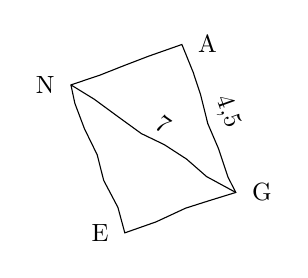
\begin{tikzpicture}[rotate=20,every node/.style={scale=0.9},scale=1]

\coordinate (N) at (0,0);
\coordinate (A) at (1.5,0);
\coordinate (G) at (1.5,-2);
\coordinate (E) at (0,-2);
\coordinate (O) at (0.75,-1); %le centre du rectangle

\draw[decorate,decoration={random steps,amplitude=1pt,segment length=10pt}] (N) node [left=3pt]{N}--(A) node [right=3pt]{A} --(G) node [right=3pt] {G}--(E) node [left=3pt] {E}--cycle;
\draw [decorate,decoration={random steps,amplitude=1pt,segment length=10pt}] (N)--(G);
\node at (.75,-1)[above,rotate=-35]{7};
\path (A)--(G) node[midway,above,rotate=-70]{4,5};

\end{tikzpicture}
